\section{}
A motor with the mass 40 kg is supported with 4 springs, each of stiffness 250 N/m as it is illustrated in following figure. The rotor is unbalanced such that the unbalanced effect is equivalent mass of 5 kg located 50 mm from the axis of rotation. (Note: There is no damping in the system.)

\begin{figure}[h]
    \centering
    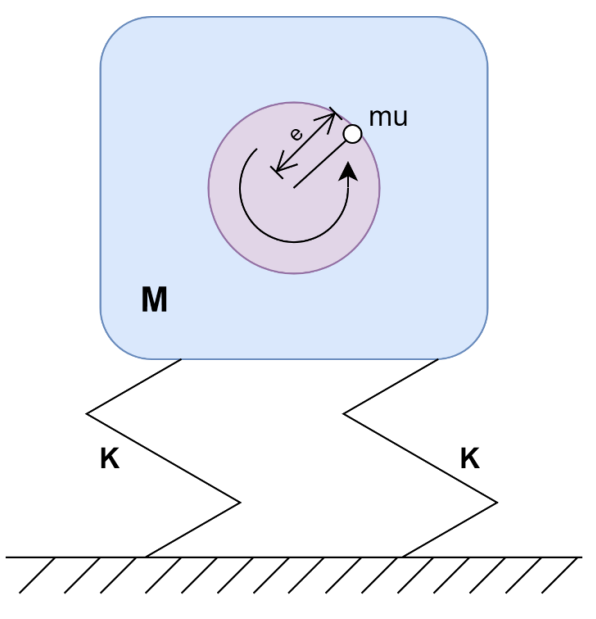
\includegraphics[width=0.5\textwidth]{Questions/Figures/q5 problem diagram.png}
\end{figure}

\begin{enumerate}[label=(\alph*)]
    \item (5 pts) Find the amplitude of vibration and the force transmitted to the foundation when the speed of motor is 1000 rpm.
    \item (5 pts.) Compare the amplitude of vibration and the transmitted force calculated in part (a) with the case that the motor is running at speed of 60 rpm.
\end{enumerate}

\subsection*{Solution}
\subsection{}
This is an undamped SDOF with rotating imbalance. The amplitude of vibration is given from (4.11), 
\begin{align*}
    \mathbb{X} &= \frac{\frac{\tilde{m} e\omega^2}{k}}{\bigg| 1- \left(\frac{\omega}{p}\right)^2 \bigg|}
\end{align*}
The natural frequency is
\begin{align*}
    p &= \sqrt{\frac{k}{m}} \\
    &= \sqrt{\frac{250 \times 4}{40}} \\
    &= 5 \text{ rad/sec}
\end{align*}
then,
\begin{align*}
    \mathbb{X} &= \frac{\frac{5 \times 50 \times 10^{-3} \times (1000 \times 2\pi/60)^2}{250 \times 4}}{\bigg| 1- \left(\frac{1000 \times 2\pi/60}{5}\right)^2 \bigg|} \\
    &= \boxed{6.264 \text{ mm}}
\end{align*}
Transmissibility is defined as
\begin{align*}
    \text{TR} :&= \frac{F_{T_{\text{max}}}}{F_{D}} \\
    &= \frac{1}{\bigg| 1- \left(\frac{\omega}{p}\right)^2 \bigg|}
\end{align*}
where the disturbing force, $F_{D} = \tilde{m} e \omega^2$. Then the transmitted force $F_{T_{\text{max}}}$ is
\begin{align*}
    F_{T_{\text{max}}} &= \frac{\tilde{m} e \omega^2}{\bigg| 1- \left(\frac{\omega}{p}\right)^2 \bigg|} \\
    &= \frac{5 \times 50 \times 10^{-3} \times (1000 \times 2\pi/60)^2}{\bigg| 1- \left(\frac{1000 \times 2\pi/60}{5}\right)^2 \bigg|} \\
    &= \boxed{6.264 \text{ N}}
\end{align*}

\subsection{}
The amplitude of vibration is then
\begin{align*}
    \mathbb{X} &= \frac{\frac{5 \times 50 \times 10^{-3} \times (60 \times 2\pi/60)^2}{250 \times 4}}{\bigg| 1- \left(\frac{60 \times 2\pi/60}{5}\right)^2 \bigg|} \\
    &= \boxed{17.042 \text{ mm}}
\end{align*}

The transmitted force is
\begin{align*}
    F_{T_{\text{max}}} &= \frac{5 \times 50 \times 10^{-3} \times (60 \times 2\pi/60)^2}{\bigg| 1- \left(\frac{60 \times 2\pi/60}{5}\right)^2 \bigg|} \\
    &= \boxed{17.042 \text{ N}}
\end{align*}